\documentclass[italian, 12pt, a4paper]{article}
\usepackage{graphicx} % Required for inserting images
\usepackage[table]{xcolor}
\usepackage[hidelinks]{hyperref} % Evita bordi colorati nei link

\setlength{\parindent}{10mm} % Imposta il rientro della prima riga di ogni paragrafo
\usepackage{xcolor}
\usepackage{titlesec}

\titleformat{\section}{\color{violet!60}\normalfont\Large\bfseries}{\thesection}{1em}{}
\titleformat{\subsection}{\color{violet!45}\normalfont\large\bfseries}{\thesubsection}{1em}{}
\titleformat{\subsubsection}{\normalfont\normalsize\bfseries\color{violet!30}}{\thesubsubsection}{1em}{}
\title{\huge{HomeProject}}
\author{Matteo Saramin, Filippo Sperandio \textit{DomusFelix} \\ {\small ITTS Vito Volterra} \\ \\ \emph{Cliente: Roberto Rossi}}

\newcommand{\version}{Version 2.5} % Definisce il comando per la versione
\date{\version\\ 15 Marzo 2025}
\begin{document}

\maketitle % Mostra titolo, autore e data

\section{Storico del Documento}
La seguente tabella riporta lo storico delle versioni del documento, includendo la versione, la data di rilascio, gli autori delle modifiche e il nome del file corrispondente.

\begin{center}
    \renewcommand{\arraystretch}{1.5} % Aumenta lo spazio verticale
    \rowcolors{2}{violet!30}{} % Alterna colori a partire dalla seconda riga
    \begin{tabular}{|c|c|c|c|}
        \hline
        \rowcolor{violet!30}
        Versione & Data & Autore & Nome Documento \\
        \hline
        1.0 & 14/03/2025 & Matteo & main.tex \\
        \hline
        2.0&25/03/2025&Matteo e Filippo & main.tex \\
        \hline
        2.5&28/03/2025&Matteo e Filippo&Main.tex\\
        \hline
    \end{tabular}\\[4mm]
\end{center}
\vspace{15mm}
\clearpage
\section{Sommario}
\begin{enumerate}
    \item \hyperref[sec:introduzione]{\Large Introduzione}
    \item \hyperref[sec:situazione]{\Large Situazione attuale}
    \item \hyperref[sec:requisiti]{\Large Requisiti Hardware \& Software}
        \begin{enumerate}
            \item Dispositivi di Illuminazione
            \item Dispositivi per la Climatizzazione
            \item Dispositivi Impianto Fotovoltaico
        \end{enumerate}
    \item \hyperref[sec:requisiti2]{\Large Specifiche Requisiti Funzionali}
        \begin{enumerate}
            \item HMI
            \item Specifiche Funzionalità
            \item Progettazione di Rete
        \end{enumerate}
\end{enumerate}
\clearpage
\section{Introduzione}\label{sec:introduzione}
L’obiettivo di questo documento è raccogliere informazioni fondamentali per la progettazione di un sistema domotico personalizzato, in grado di soddisfare le esigenze specifiche del cliente.\\[1.5mm]Il nostro progetto prevede lo sviluppo di un’interfaccia grafica interattiva che consentirà agli utenti di controllare in modo semplice ed efficace le funzionalità della propria abitazione. L’idea centrale è offrire un sistema intuitivo, accessibile da più dispositivi e in grado di migliorare il comfort, la sicurezza e l’efficienza energetica della casa.\\[1.5mm]
Per garantire che il sistema realizzato sia il più possibile aderente alle necessità del cliente, abbiamo strutturato un questionario mirato, suddiviso in diverse sezioni. Questo questionario è stato elaborato per raccogliere dettagli sulla configurazione dell’abitazione, i dispositivi domotici desiderati, le funzionalità ritenute più importanti e le preferenze riguardanti l’interfaccia utente.
Le informazioni fornite dal cliente ci permetteranno di sviluppare un sistema domotico su misura, ottimizzando la disposizione dei dispositivi, i parametri di controllo e l’interazione con il sistema. Inoltre, l’analisi delle risposte ci aiuterà a progettare un’interfaccia grafica chiara e funzionale, organizzata in base alle diverse zone della casa e alle principali operazioni disponibili.\\[1.5mm]
La comunicazione con il cliente è un elemento essenziale per il successo del progetto, e questo documento rappresenta un primo passo cruciale per garantire che il prodotto finale risponda alle aspettative e necessità dell’utente.
\clearpage
\section{Situazione attuale}\label{sec:situazione}
\subsection{Versione 1.0}
\begin{quote}
In questa prima versione abbiamo definito la struttura generale della documentazione, compresa di questo documento e del questionario fornitore-cliente.  Nei primissimi giorni abbiamo definito generalmente l'impostazione dell'interfaccia grafica, senza addrentrarci però nei dettagli, per avere una maggiore flessibilità nelle succesive giornate.
\end{quote}
\subsection{Versione 2.0}
\begin{quote}
    In questa seconda fase ci siamo focalizzati nel progettare più dettagliamente l'interfaccia grafica, in un primo momento con una rappresentazione grafica realizzata congiuntamente, e succesivamente definendola con un sito web in locale, tramite linguaggio \emph{HTML, CSS e Javascript}. Inoltre la stesura della documentazione è proseguita, in particolare con il questionario, dopo anche una revisione in cooperazione con la prof. \emph{Tollot}. Abbiamo scelto GitHub per condividere il progetto, in modo da facilitare la collaborazione, tracciare le modifiche e mantenere una copia centralizzata del nostro lavoro.
\end{quote}
\subsection{Versione 2.5}
\begin{quote}
    All'avvicinarsi della scadenza per l'interfaccia grafica e documentazione abbiamo concluso la stesura della documentazione, individuando gli ultimi requisiti software e hardware, e le funzionalità richieste dall'utente. Abbiamo progettato la planimetria della casa, tramite il software \emph{RoomSketcher}, scelto per la sua facilità d'uso e i modelli predefiniti, che abbiamo adattato alle nostre esigenze, e implementato nell'interfaccia grafica. Infine abbiamo terminato l'interfaccia grafica, suddividendola in due implementazioni, una per i pannelli presenti in ogni stanza, e una per i dispositivi, quali computer o telefoni.
\end{quote}
\clearpage
\section{Requisiti Hardware \& Software}\label{sec:requisiti}
Per un coretto ed efficiente funzionamento dell'intero sistema domotico della casa del nostro cliente, in relazione alle sue richieste e necessità, abbiamo individuato i seguenti requisiti hardware e software.
\begin{enumerate}
    \item L'interfacci grafica deve essere utilizzata dal cliente, e richiede che sia chiara, semplice e intuitiva, in modo da modificare i parametri della casa a suo piacimento. Questi parametri sono: la temperatura, l'illuminazione, l'automazione delle finestre, l'irrigazione del giardino e il sistema d'allarme.
    \item L’interfaccia deve adattarsi a diversi dispositivi, funzionando efficacemente su desktop e mobile.
    \item Le modifiche apportate dall’utente devono essere applicate in tempo reale e riflesse nel sistema senza ritardi eccessivi.
    \item Deve essere presente un pannello di controllo in ogni stanza della casa, con ovviamente la possibilità di modificare i relativi parametri di quella stanza, come illuminazione e temperatura.
    \item Il sistema deve supportare i dispositivi intelligenti che implementano le funzionalità scelte dal'utente.
    \item Il sistema deve permettere di accendere e spegnere le luci in ogni stanza, sia tramite l'interfaccia grafica che fisicamente tramite un pulsante; inoltre sono implementanti delle automazioni, in relazionea a sensori e orari.
    \item Il sistema deve permettere di gestire la temperatura della casa, tramite gli adeguati dispositivi di riscaldamento e raffreddamento.
    \item Il sistema deve supportare l'impianto fotovoltaico, munito di 4 pannelli solari e una batteria, per una maggiore efficienza e garantendo l’utilizzo di energia completamente rinnovabile.
    \item Deve essere possibile verificare la produzione energetica dei pannelli fotovoltaici. Di conseguenza è necessario visualizzare anche la percentuale della batteria. Gli altri parametri necessari sono il consumo energetico dell’intera casa e la temperatura interna e esterna della casa.
\end{enumerate}
\clearpage
\section{Dispositivi Installati}
Per garantire un sistema domotico efficiente e funzionale, è stata effettuata una selezione attenta dei dispositivi hardware. La scelta è stata guidata dall’obiettivo di ottimizzare l’integrazione tra i vari componenti, garantendo affidabilità, efficienza energetica e semplicità d’uso per l’utente finale.
Nelle sezioni seguenti verranno illustrati i dispositivi adottati, per implementare le funzionalità dell'illuminazione, gestione della temperatura, automazione delle finestre, irrigazione, impianto fotovoltaico e sistema d'allarme.
\subsection{Illuminazione}
\subsubsection{1° Lampada Pendente}
Abbiamo scelto come corpo illuminante principale un lampadario pendente a LED, di forma sferica e paralume in tessuto ignifugo, adatta ad un'illuminazione ottimale di vasti ambienti o camere.
\begin{quote}
    \begin{enumerate}
        \item Sorgente Luminosa: \emph{LED}.
        \item Potenza: \emph{50W}.
        \item Flusso luminoso: \emph{4000 lumen}.
        \item Temperatura Colore: \emph{4000K}.
        \item D = \emph{50cm} $H_t = \emph{190cm}$
    \end{enumerate}
\end{quote}
\begin{figure}[h!]
    \centering
    \begin{minipage}{0.45\textwidth}
        \centering
        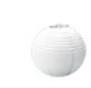
\includegraphics[width=0.6\linewidth]{img/lampada.png} % modifica con il percorso della tua prima immagine
        \caption{Vista 3D}
    \end{minipage} \hfill
    \begin{minipage}{0.45\textwidth}
        \centering
        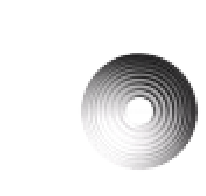
\includegraphics[width=0.6\linewidth]{img/lampada-top.png} % modifica con il percorso della tua seconda immagine
        \caption{Vista dall'alto}
    \end{minipage}
\end{figure}
\hrule
\subsubsection{2° Lampada da Muro}
Abbiamo scelto come secondo corpo illuminante un lampadario pendente a LED, di forma sferica e paralume in tessuto ignifugo, adatta ad un'illuminazione ottimale di vasti ambienti o camere.
\begin{quote}
    \begin{enumerate}
        \item Sorgente Luminosa: \emph{LED}.
        \item Potenza: \emph{28W}.
        \item Flusso luminoso: \emph{4000 lumen}.
        \item Temperatura Colore: \emph{3000K}.
        \item L = \emph{60cm}; $H_t = \emph{150cm};$
    \end{enumerate}
    \vspace{-40pt}
\end{quote}
\begin{figure}[h!]
    \centering
    \begin{minipage}{0.45\textwidth}
        \centering
        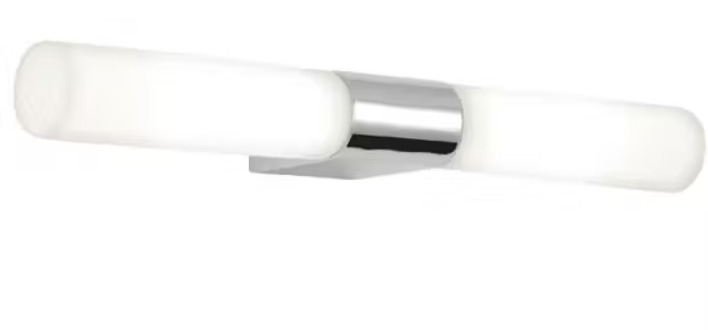
\includegraphics[width=\linewidth]{img/Lampada_muro.png} % modifica con il percorso della tua prima immagine
        \caption{Vista 3D}
    \end{minipage} \hfill
    \begin{minipage}{0.45\textwidth}
        \centering
        
\includegraphics[width=\linewidth]{img/lampada-muro-top.png} % modifica con il percorso della tua seconda immagine
        \caption{Vista dall'alto}
    \end{minipage}
\end{figure}
\hrule
\subsubsection{3° Lampada da Tavolo}
Come terzo corpo illuminante abbiamo scelto una lampada da tavolo, combaciando perfettamente un ottimo oggetto di design e una illuminazione soffusa nelle ore notturne perfetta per la lettura o scrittura.
\begin{quote}
    \begin{enumerate}
        \item Sorgente Luminosa: \emph{LED}.
        \item Potenza: \emph{100W}.
        \item Flusso luminoso: \emph{1600 lumen}.
        \item Temperatura Colore: \emph{2700K}.
        \item D = \emph{42cm}; H = \emph{62cm};
    \end{enumerate}
\end{quote}
\begin{figure}[h]
    \centering
    \begin{minipage}{0.45\textwidth}
        \centering
        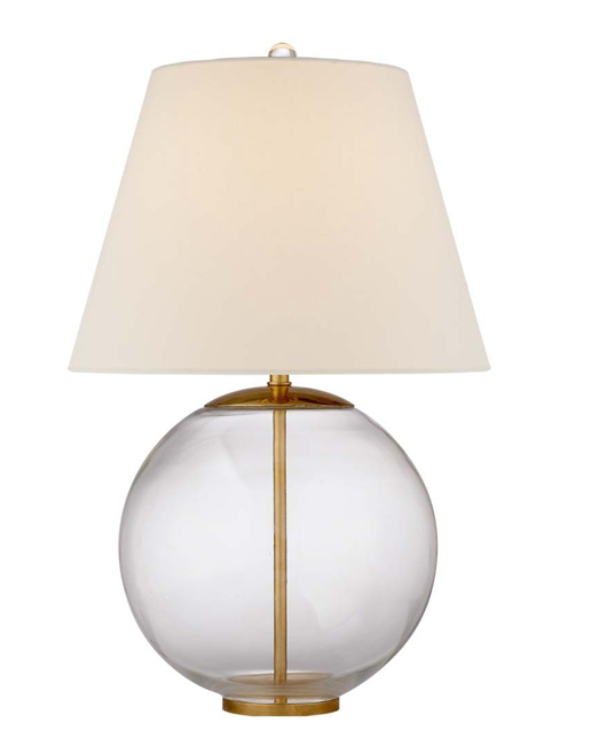
\includegraphics[width=0.5\linewidth]{img/lampada-tavolo.png} % modifica con il percorso della tua prima immagine
        \caption{Vista 3D}
    \end{minipage} \hfill
    \begin{minipage}{0.45\textwidth}
        \centering
        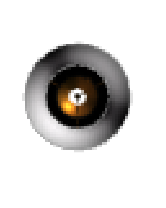
\includegraphics[width=0.5\linewidth]{img/lampada-tavolo-top.png} % modifica con il percorso della tua seconda immagine
        \caption{Vista dall'alto}
    \end{minipage}
\end{figure}
\hrule
\clearpage
\subsection{Dispositivi per la Climatizzazione}
\subsubsection{1° Dispositivo Termoregolatore}
Ho scelto di installare un condizionatore con funzione sia di raffreddamento che di riscaldamento per garantire un comfort ottimale tutto l'anno, ottimizzando l'efficienza energetica e riducendo i costi rispetto a soluzioni separate.
\begin{quote}
    \begin{enumerate}
        \item Capacità di Raffredamento: \emph{9000 BTU}
        \item Capacità di Riscaldamento: \emph{7000 BTU}
        \item Efficienza Energetica: \emph{A++}
        \item W = \emph{48cm};  = \emph{85cm}; Peso: \emph{10kg}; 
    \end{enumerate}
\end{quote}
\begin{figure}[h!]
    \centering
    \begin{minipage}{0.45\textwidth}
        \centering
        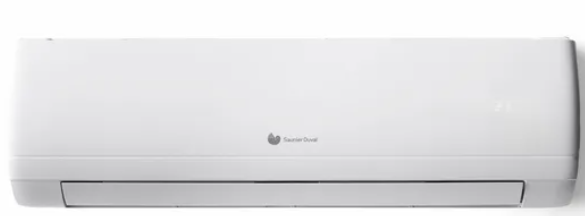
\includegraphics[width=0.7\linewidth]{img/condizionatore.png} % modifica con il percorso della tua prima immagine
        \caption{Vista 3D}
    \end{minipage} \hfill
    \begin{minipage}{0.45\textwidth}
        \centering
        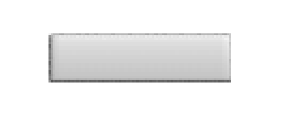
\includegraphics[width=0.7\linewidth]{img/condizionatore-top.png} % modifica con il percorso della tua seconda immagine
        \caption{Vista dall'alto}
    \end{minipage}
\end{figure}
\hrule
\subsubsection{2° Dispositivo di Riscaldamento}
Abbiamo scelto di installare un pannello riscaldante in bagno per garantire un riscaldamento più uniforme e discreto. Inoltre, il pannello offre un'alternativa più pulita e sicura rispetto ai tradizionali radiatori, riducendo al minimo l'accumulo di polvere e aumentando l'efficienza energetica.
\begin{quote}
    \begin{enumerate}
        \item Capacità di Riscaldamento: \emph{7000 BTU}
        \item Efficienza Energetica: \emph{A++}
        \item W = \emph{102cm}; L = \emph{64cm}; Peso: \emph{7kg}; 
    \end{enumerate}
\end{quote}
\vspace{-15px}
\begin{figure}[h]
    \centering
    \begin{minipage}{0.45\textwidth}
        \centering
        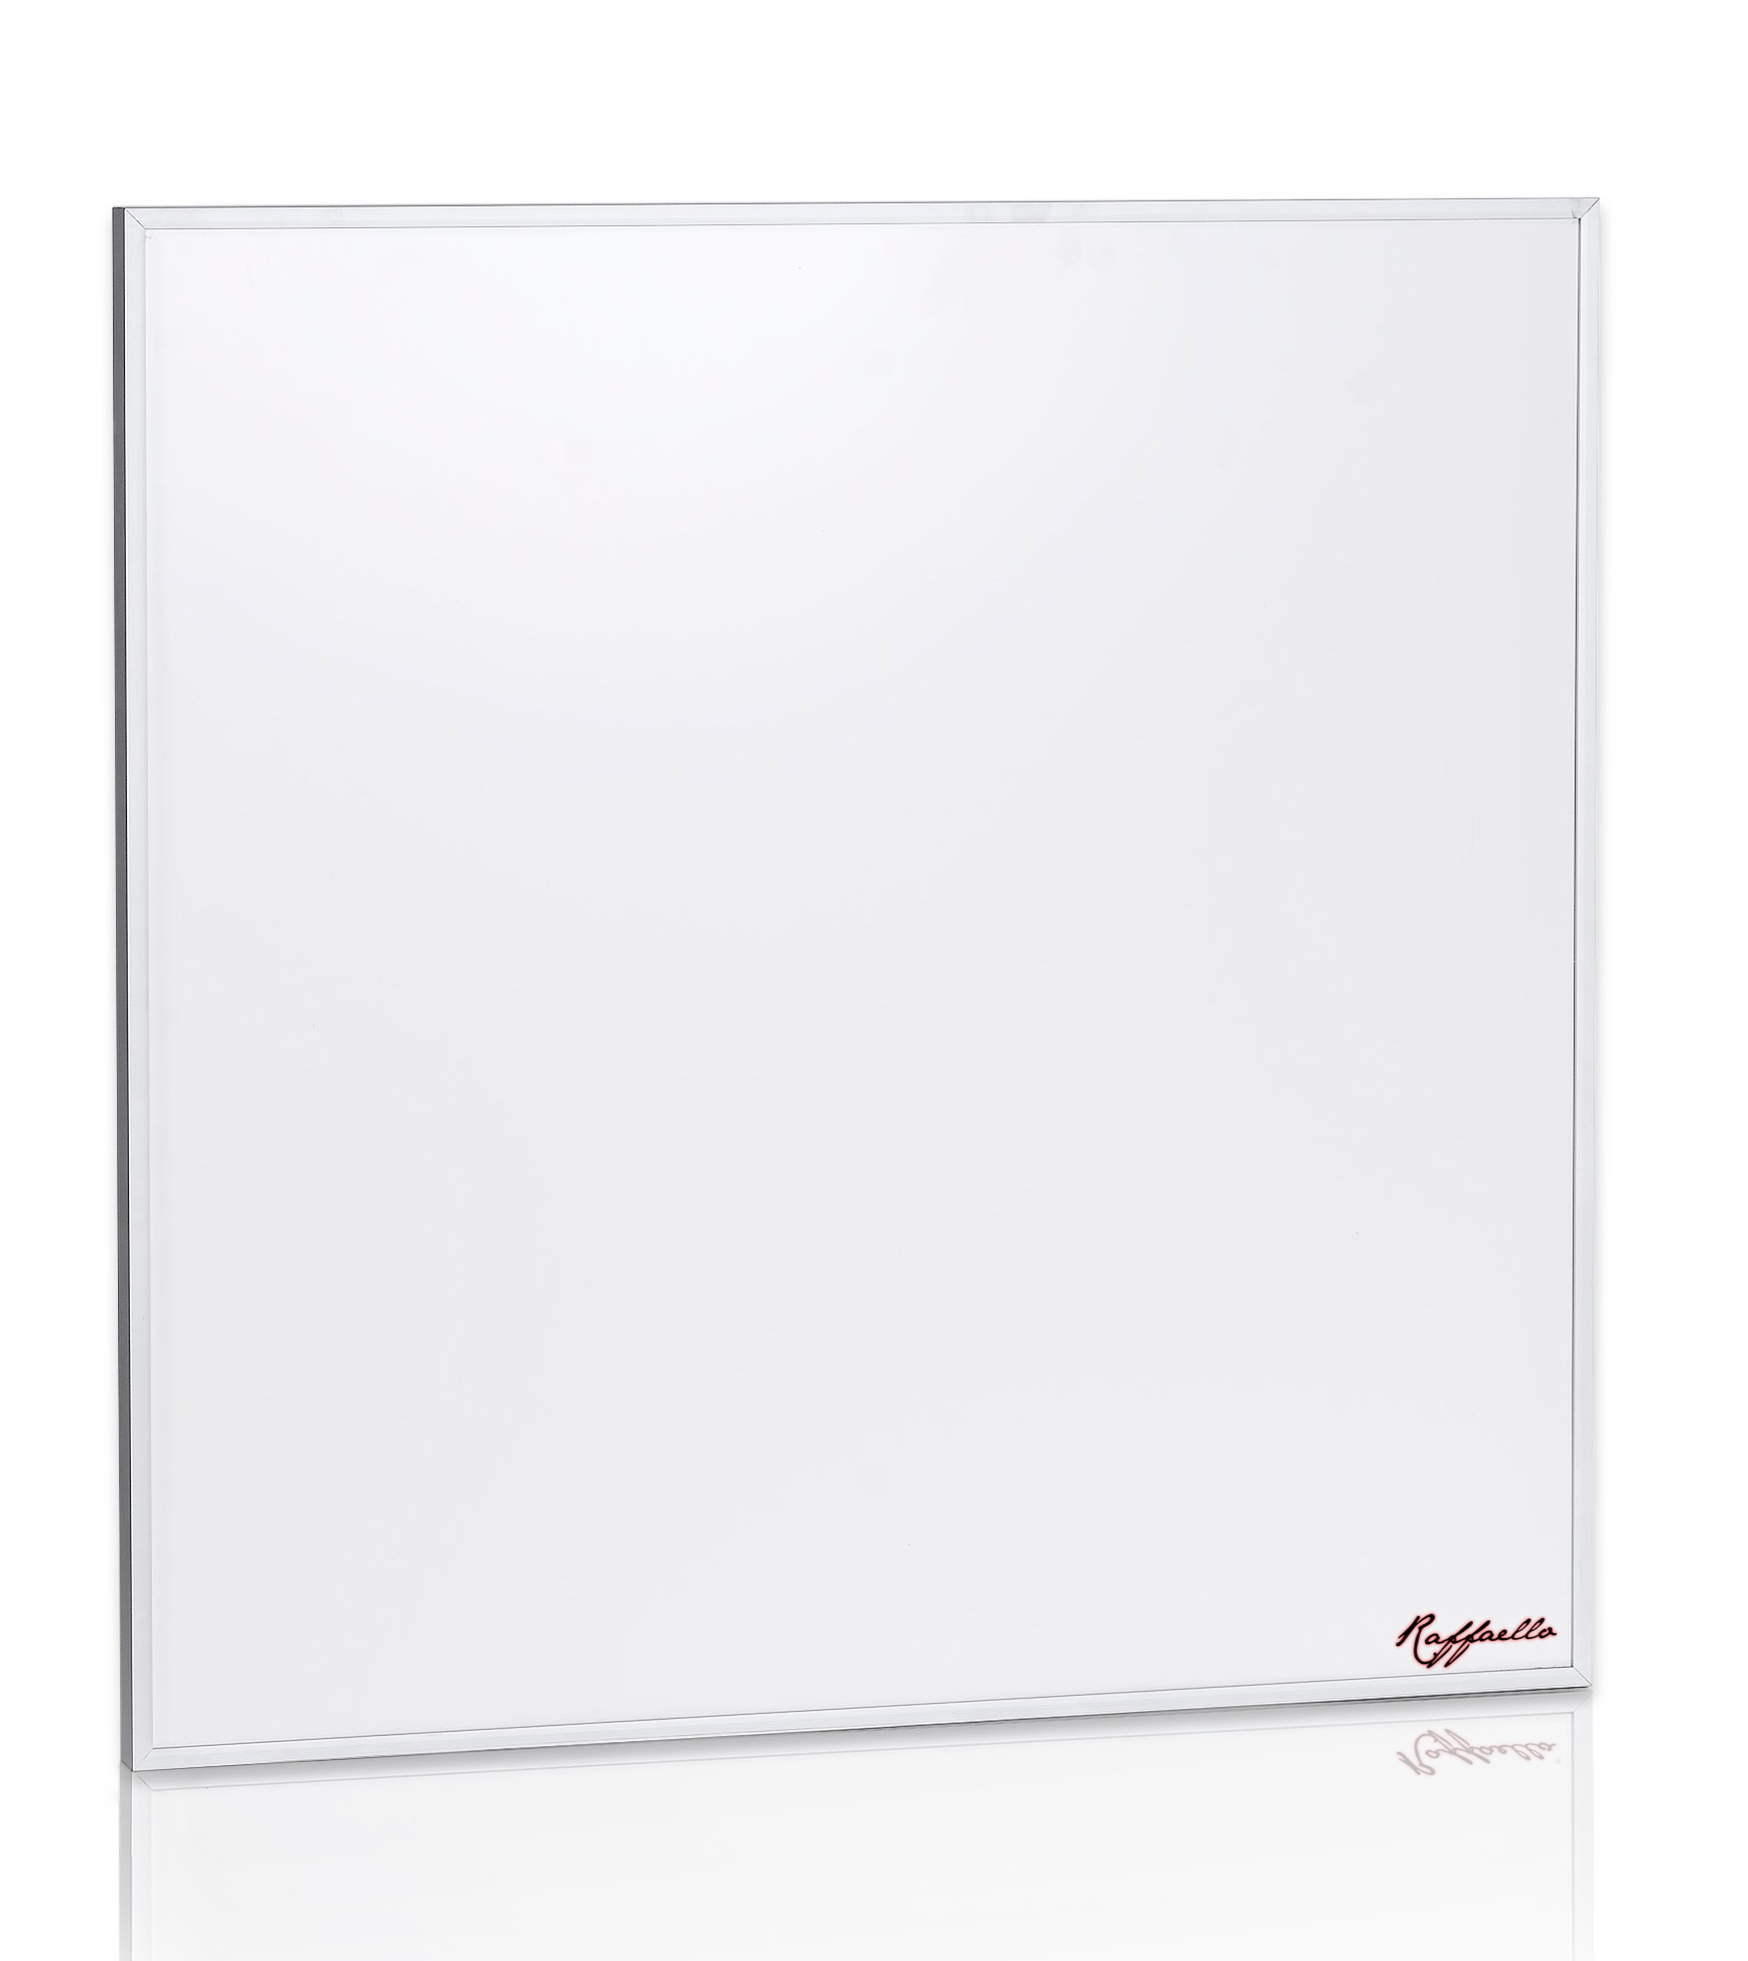
\includegraphics[width=0.4\linewidth]{img/pannelo.png} % modifica con il percorso della tua prima immagine
        \caption{Vista 3D}
    \end{minipage} \hfill
    \begin{minipage}{0.45\textwidth}
        \centering
        
\includegraphics[width=0.4\linewidth]{img/panello-top.png} % modifica con il percorso della tua seconda immagine
        \caption{Vista dall'alto}
    \end{minipage}
\end{figure}
\clearpage
\subsection{Dispositivi Impianto Fotovoltaico}
\subsubsection{Pannello Fotovoltaico}
Ho scelto il pannello JA Solar Black Frame da 415W per la sua alta efficienza e affidabilità. La potenza di 415W garantisce una buona produzione di energia, mentre la garanzia di 12 anni assicura una lunga durata. Il pannello utilizza tecnologia monocristallina, offrendo un'alta efficienza nella produzione di energia solare anche nelle ore con scarsa luminosità.
\begin{quote}
    \begin{enumerate}
        \item Potenza nominale: \emph{410W}.
        \item N° di Celle: \emph{108 ($6\times 18$)}.
        \item T° Operativa: \emph{-40° - +85°}.
        \item Garanzia: \emph{12 anni}.
        \item L = \emph{172cm}; W = \emph{97cm}; peso: \emph{16.7kg};
    \end{enumerate}
\end{quote}
\vspace{-15px}
\begin{figure}[h]
    \centering
    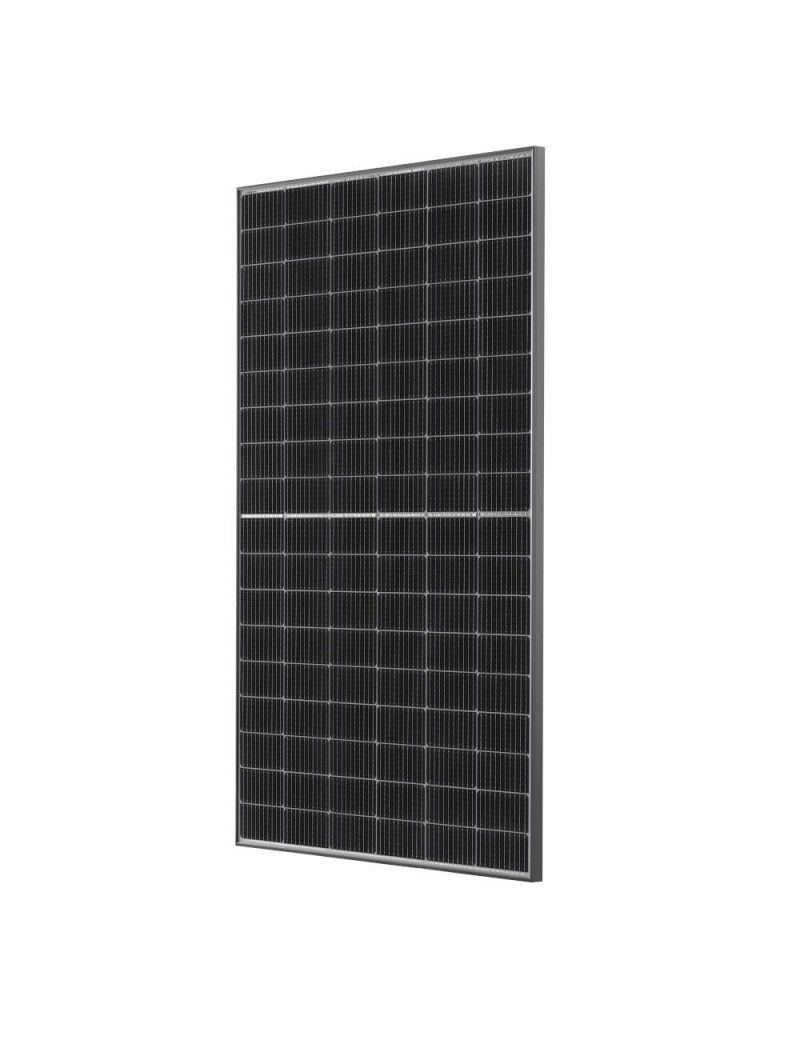
\includegraphics[width=0.6\linewidth]{img/pannello-solare.png}
    \caption{Vista 3D}
    \label{fig:pannello-solare}
\end{figure}
\subsubsection{Batteria}
La scelta della batteria per l'impianto fotovoltaico è stata dettata da parametri rigurdanti una totale sicurezza, data la sensibilità del dispositivo. Inoltre assicura un'alimentazione della casa anche nelle ore con scarsa o nulla produzione energetica.
\begin{quote}
    \begin{enumerate}
        \item Energia Totale: \emph{10300Wh}.
        \item potenza uscita Contnua: \emph{5000W}.
        \item Grado di Protezione: \emph{IP55}.
        \item T° Operativa: \emph{-10° - +50°}.
        \item Garanzia: \emph{10 anni}.
        \item L = \emph{1179cm}; W = \emph{250cm}; peso: \emph{121kg};
    \end{enumerate}
\end{quote}
\vspace{-15px}
\begin{figure}[h]
    \centering
    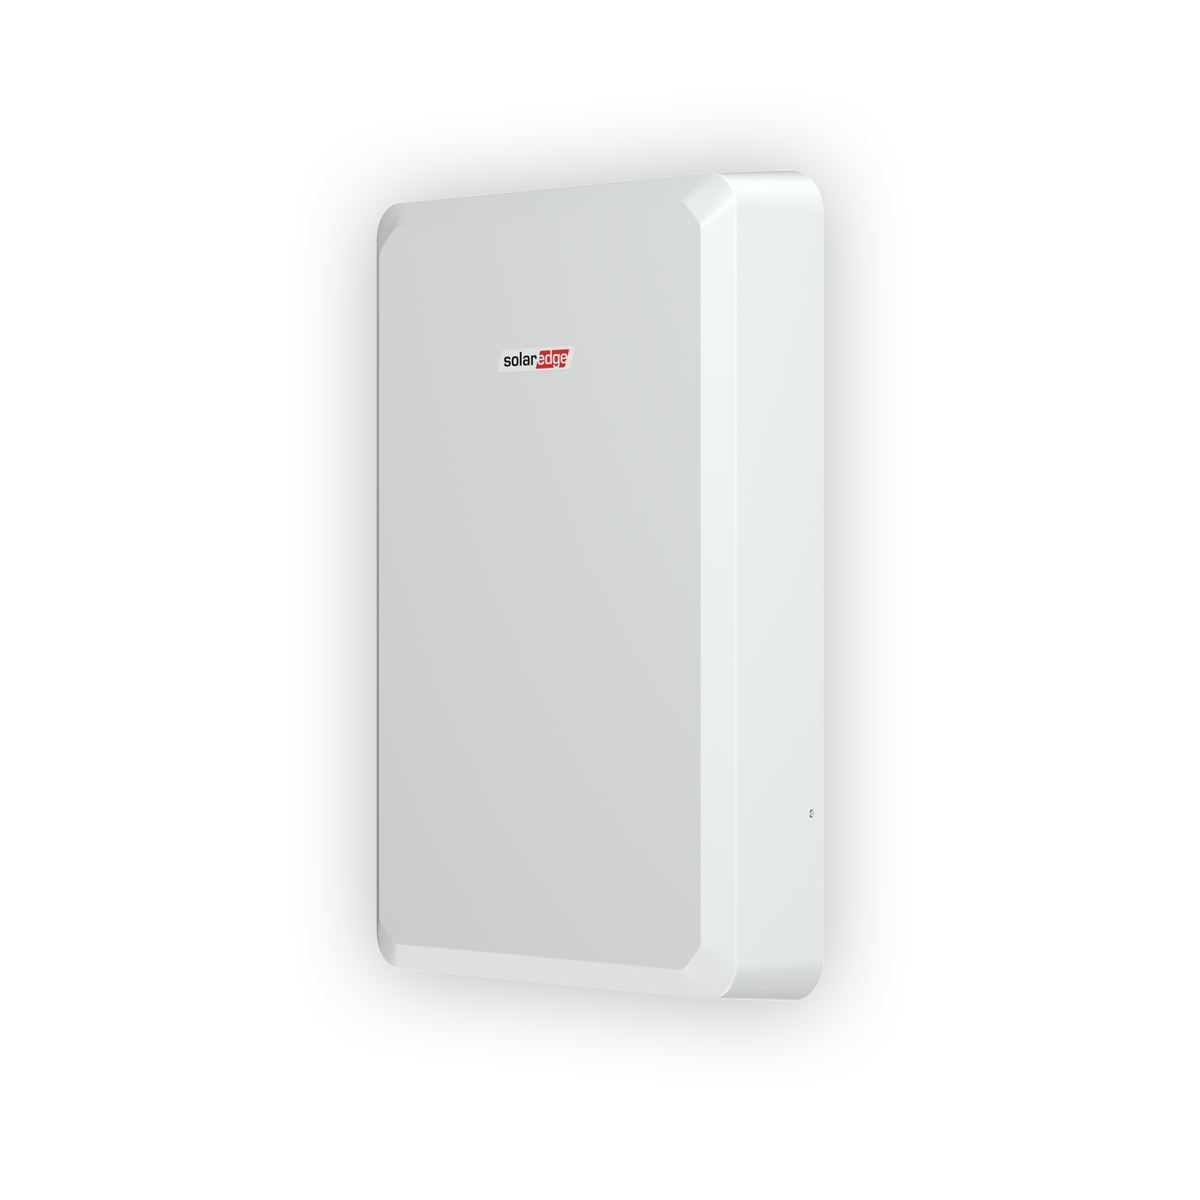
\includegraphics[width=0.6\linewidth]{img/batteria.png}
    \caption{Vista 3D}
    \label{fig:batteria}
\end{figure}
à
    % Specifica Requisiti Funzionali
\clearpage
\section{Specifica Requisiti Funzionali}\label{sec:requisiti2}
\subsection{HMI - Human Machine Interface}
Il cliente richiede un’interfaccia grafica (HMI) accessibile da più dispositivi, tra cui computer, telefoni, un tablet e pannelli di controllo installati in ogni stanza. Questi dispositivi devono garantire un'esperienza un uso ottimale, un'interfaccia responsive che si adatti automaticamente alle diverse dimensioni dello schermo e che mantenga una navigazione fluida e intuitiva.  I pannelli di controllo posizionati strategicamente in ogni stanza della casa, devono consentire la gestione dei parametri della relativa stanza, di cui: illuminazione, temperatura, stato delle finestre, irrigazione e il sistema d’allarme. Gli altri dispositivi, di cui telefoni, computer e un tablet devono invece rappresentare lo stato generale della casa, con comunque la possibilità di interagire con il sitema domotica di ogni singola stanza.\\[1.5mm]
Un aspetto fondamentale dell’HMI è il monitoraggio dell’impianto fotovoltaico, che deve fornire in tempo reale dati sulla produzione energetica, la percentuale di carica della batteria e il consumo energetico dell’abitazione. Il cliente desidera una rappresentazione chiara e dettagliata di queste informazioni, con grafici intuitivi e indicatori che permettano di valutare rapidamente l’efficienza del sistema.\\[1.5mm]
La struttura dell’interfaccia grafica richiesta dall’utente è la seguente: un prima rappresentazione visiva dei parametri fondamentali della casa domotica, visti in precedenza, successivamente una rappresentazione dell’intera casa, munita degli apparati intelligenti, in modo da modificare lo stato di essi. Infine un’ultima sezione con alcune specifiche del complesso della casa; di cui queste sono richieste esplicitamente dall’utente: Consumo energetico dell’intera casa, produzione in kW dell’impianto fotovoltaico e lo stato di carica della batteria, e la temperature esterna ed interna.\\[1.5mm]
La modalità con cui l’utente approccia con il sistema è appunto attraverso l’interfaccia grafica, deve quindi quest’ultima essere semplice, intuitiva, senza eccessivi ritardi e un’organizzazione delle funzioni che renda il controllo della casa semplice e immediato, anche per utenti senza particolari competenze tecniche.
\subsection{Specifiche Funzionalità}
\ldots
\subsection{Progettazione di Rete}
Il cliente ha richiesto un sistema che implementasse le funzionalità precedentemente discusse, tramite una rete da noi progettata e realizzata. Abbiamo implementato la possibilità di interagire con i dispositivi IoT, in modo intuitivo tramite i dispostivi adatti. 
\subsubsection{Elenco dei Dispositivi}
\begin{enumerate}
    \item luci
    \item AC
    \item radiatori
    \item Irrigatori
    \item Sirena
    \item Sensore Vento
    \item Sensore Movimento
\end{enumerate}
\clearpage
\end{document}
